\section{概要}
本プロジェクトでは、雑多な環境下で人追従でき、ロボットの最大直進速度で追従するため、
2D-LiDARの距離データとリアルタイム物体検出アルゴリズムであるYOLOv8を用いた人追従システムを開発する。
本プロジェクトで提案する人追従システムは、追従対象者のみがいる雑多な環境を想定している。
雑多な環境では、人の脚部と形状が類似している椅子やポールなどの物体をランダムに多数
設置している。2D-LiDARから提供される距離データを俯瞰画像に変換し、
学習したYOLOv8と俯瞰画像を用いて追従対象者の検出をする。追従対象者の検出のみでは、
周囲の物体を両脚部と誤検出する可能性があるため、追従目標の特定処理をシステムに組み込む
ことで、正確に追従対象者を追従することを実現する。

\section{要求仕様}
本プロジェクトでは、雑多な環境下で人追従でき、ロボットの最大直進速度で追従できる人追従システムの
開発を目的としているため、以下の構成で要求仕様を設定する。
使用するロボットは、2023年に開催されたRoboCup 2023で開発したロボットである
Happy Eduを使用する。Happy Eduのロボット台車は、ROBOTIS社のTurtleBot3 Big Wheelであり、
ロボット台車の前方に2D-LiDARを搭載している。
2D-LiDARは、北陽電機株式会社のUTM30-LXを使用しており、ロボットに搭載するPCは、
NVIDIA GeForce RTX 4070 8GB を搭載しているノートPCを選定した。\\ \indent
以上の構成で以下の要求仕様を設定する。\\

\begin{enumerate}
\item 2D-LiDARのデータで人追従ができる \\
\item 雑多な状態の空間でも人追従ができる \\
\item 0.5[m/s]以下の歩行速度で追従する \\
\end{enumerate}

\section{システム構成}
本プロジェクトでは、Fig. \ref{System configuration chart}のような人追従システムを提案する。
2D-LiDARから提供される距離データを俯瞰画像に変換し、YOLOv8のリアルタイム物体検出モデルにより
人の両脚部分を検出する。YOLOv8による人の両脚部分の検出は、別の物体を誤検出することがあるため、
追従対象の特定処理を実装している。追従対象の特定後、ロボットが追従すべき目標座標を生成し、
ロボットから目標座標までの距離と角度の偏差を収束させるため、PID制御によりロボット台車を制御する。

\begin{figure*}[h]
    \begin{center}
    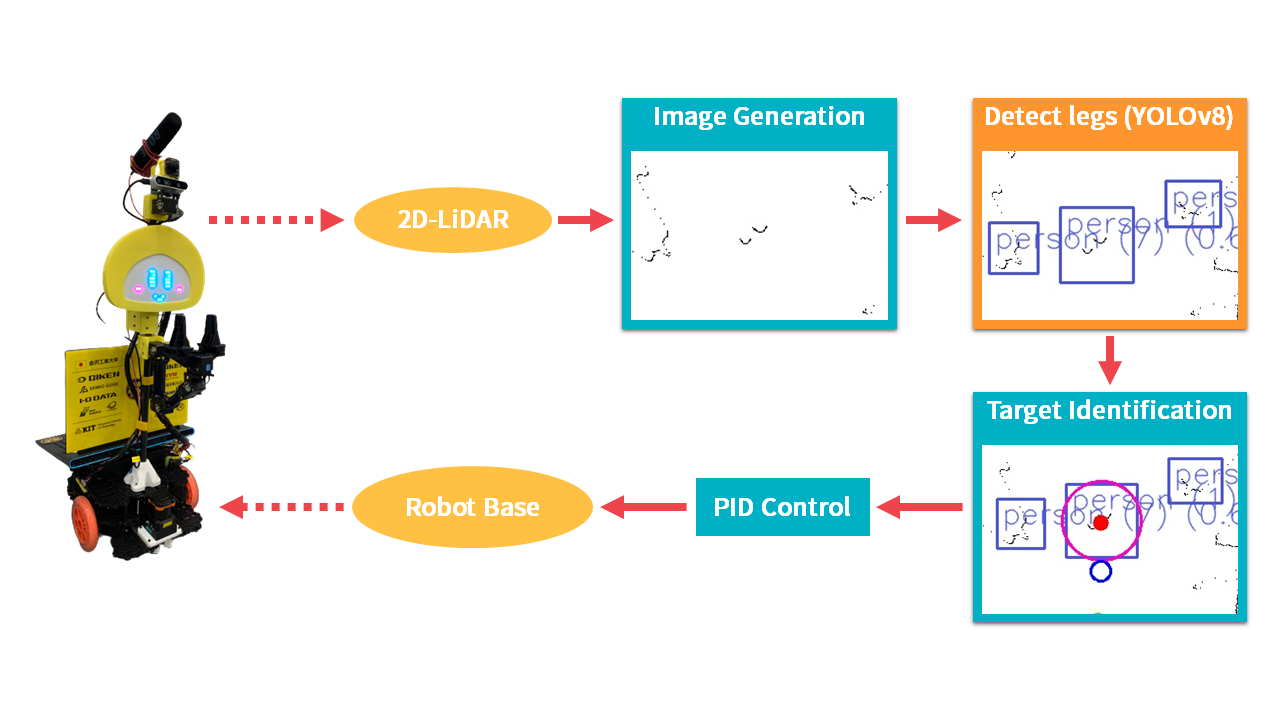
\includegraphics[height=90mm,clip]{figure/System-configration-chart.png}
    \caption{System configuration chart}
    \label{System configuration chart}
    \end{center}
\end{figure*}

\section{ソフトウェア構成}
ロボット用ノートPC内のソフトウェア構成をFig. \ref{Software configuration diagram}に示す。
ロボット用ノートPCのオペレーティングシステムにはUbuntu22.04を使用し、ミドルウェアには
Robot Operationg System 2 (以下、ROS2)を用いている。ロボットのソフトウェア開発には、
主にPython言語を使用し、YOLOv8のROS2パッケージにはyolov8\_rosパッケージを用いている。
今回開発した人追従システムは、ROS2パッケージになっており、Fig. \ref{Software configuration diagram}
のfollow\_me Package上の構成となっている。\\ \indent
各ノードの処理内容は以下の通りである。

\begin{itemize}
    \item YOLOv8 Nodes: 俯瞰画像から人の両脚部分を検出する。
    \item laser\_to\_image Node: 2D-LiDARの距離データを俯瞰画像に変換する。
    \item person\_detector Node: 推論結果をもとに、追従対象を特定し目標座標を生成する。
    \item base\_controller Node: 目標座標までの距離と角度の偏差をPID制御により収束させる。
\end{itemize}

\begin{figure*}[h]
    \begin{center}
    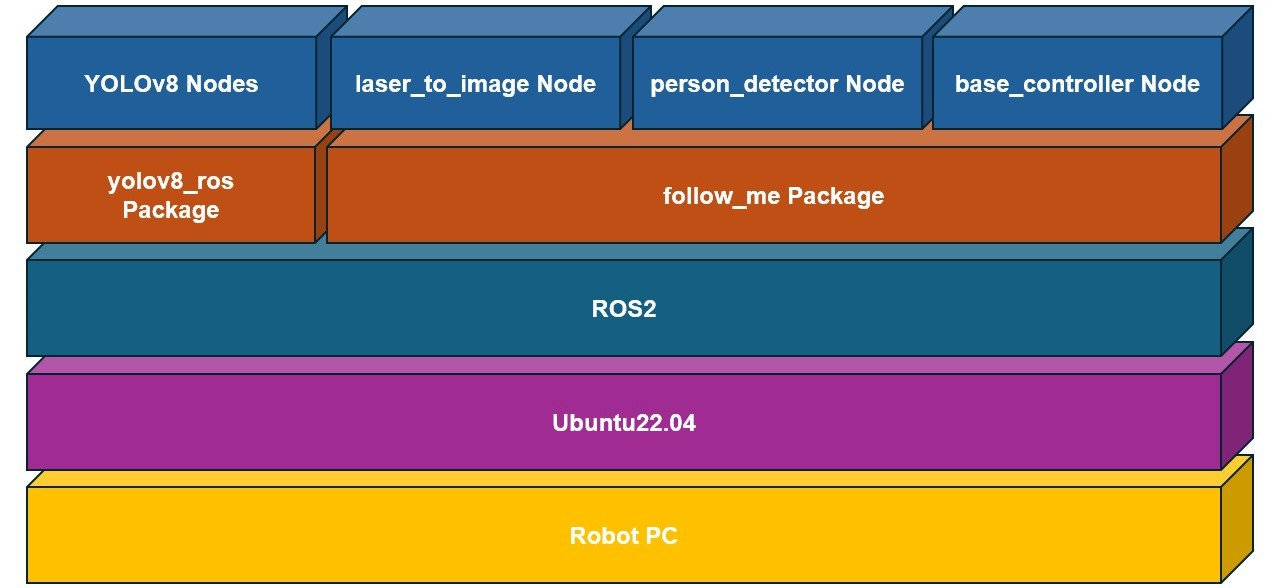
\includegraphics[height=80mm,clip]{figure/Software.jpg}
    \caption{Software configuration diagram}
    \label{Software configuration diagram}
    \end{center}
\end{figure*}

\clearpage

\section{データセットの作成}
2D-LiDARのデータをFig. \ref{Example of an overhead view image}のように俯瞰画像へ変換し、
データセットを作成する。データセットを作成するときの環境は、ロボットが静止した状態において、
タイトパンツとワイドパンツを着用している2人が大股や小股などで歩行し、歩行パターンはランダムである。
これを5分間行い、俯瞰画像をトピック通信で発信し続け、ROS2 Bagを保存する。ROS2 Bagは、
ROS2におけるトピックの保存機能である。ROS2 Bagのデータをから12032枚の画像データを生成し、
人の脚部をpersonクラスとしてアノテーションを行った。Fig. \ref{Example data sets}
にデータセットの例を示す。
また、データセットには、画像の回転処理、モザイク処理、2枚の画像を合成し、新しく1枚の画像を
生成するMix Up処理をすることでデータ拡張を行った。

\begin{figure*}[h]
    \begin{center}
    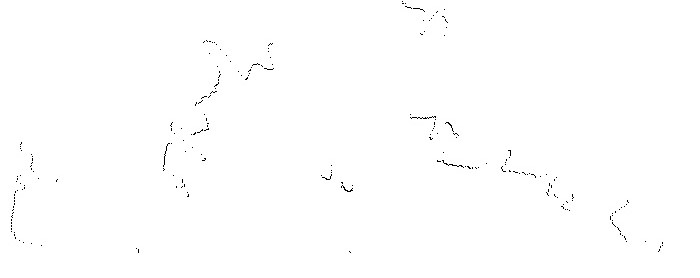
\includegraphics[height=50mm,clip]{figure/laser_img_232.jpg}
    \caption{Example of an overhead view image}
    \label{Example of an overhead view image}
    \end{center}
\end{figure*}

\begin{figure*}[h]
    \begin{center}
    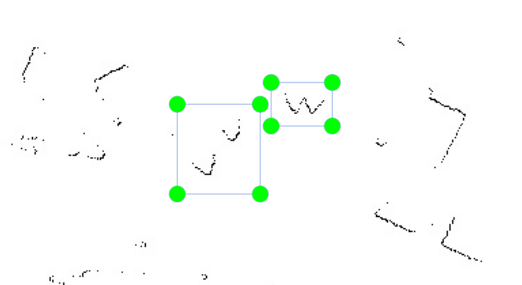
\includegraphics[height=60mm,clip]{figure/Example-data-sets.png}
    \caption{Example data sets}
    \label{Example data sets}
    \end{center}
\end{figure*}

\section{YOLOv8による学習}
作成したデータセットとYOLOv8を用いて人の両脚検出器を作成する。
学習には、リアルタイム物体検出アルゴリズムであるYOLO (You Only Look Once)を使用し、
学習モデルの初期重みは、ロボットに搭載するノートPCの性能が高いため、最もパラメータ数
の多いYOLOv8xを選定した。学習するPCは、NVIDIA GeForce RTX 4090 16GBを搭載している
PCを使用し、バッチサイズは12、エポック数は500で学習を行った。過学習を防ぐため、
過学習が発生する直前または発生したらすぐに学習を終了させる処理を100エポック以降で設定した。
学習結果は、Fig. \ref{Training results}とFig. \ref{Example of inference results with YOLOv8 using learned weights}
のようになっており、推論結果が90[\%]を超えていることが分かる。

\begin{figure*}[h]
    \begin{center}
    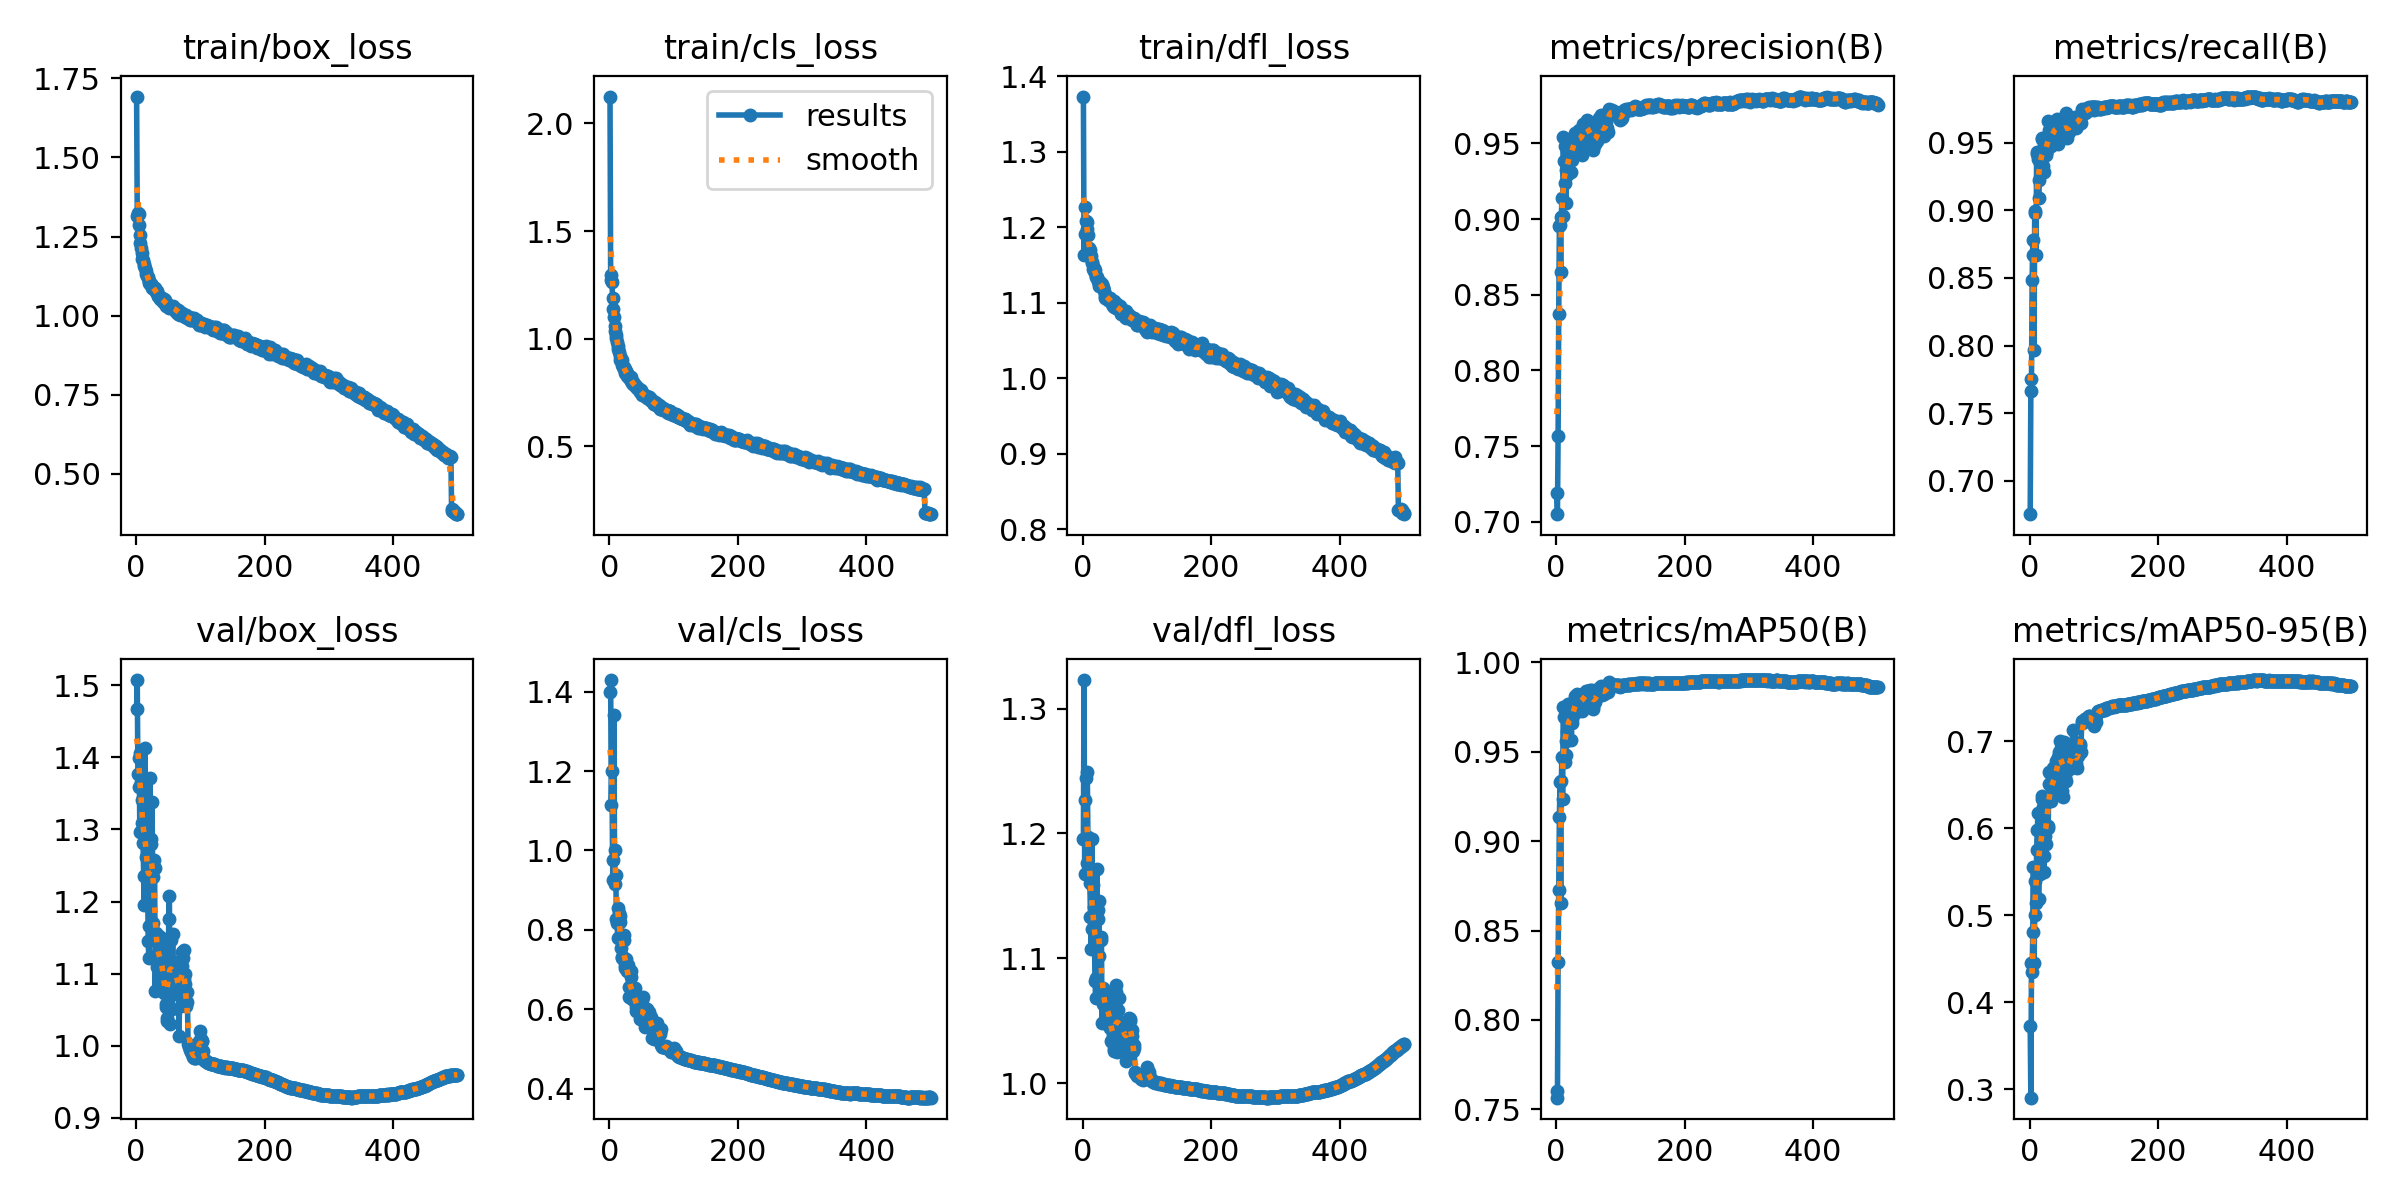
\includegraphics[height=70mm,clip]{figure/yolov8-train-results.png}
    \caption{Training results}
    \label{Training results}
    \end{center}
\end{figure*}

\begin{figure*}[h]
    \begin{center}
    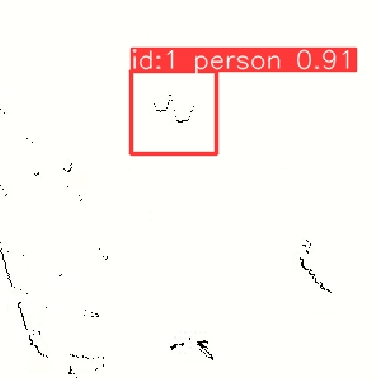
\includegraphics[height=60mm,clip]{figure/yolov8_laser_img.png}
    \caption{Example of inference results with YOLOv8 using learned weights}
    \label{Example of inference results with YOLOv8 using learned weights}
    \end{center}
\end{figure*}

\section{追従目標の特定}
YOLOv8による推論結果を用いて追従目標の特定をする。
YOLOv8には、Byte Trackなどの追跡アルゴリズムが標準機能で搭載されており、検出した物体
にIDを付与することができる。しかし、1度検出を外れ、再度同じ物体が検出されてもIDが変わって
しまうという問題がある。そこで、動的検出範囲を実装することで特定の追従目標を追従し続ける。\\ \indent
本プロジェクトで実装した追従目標の特定方法をFig. \ref{Target identification methods}
に示す。1フレーム前における追従目標のバウンディングボックスを中心とした、半径0.5[m]の
円型範囲を現在のフレームに設定し、範囲内にバウンディングボックスの中心があればそれを
追従対象とする。円型範囲の半径は、ROS2のパラメータ通信で実装しているため、値を動的に変更
可能であり、歩行速度に合わせて円型範囲を拡大縮小することが可能である。

\begin{figure*}[h]
    \begin{center}
    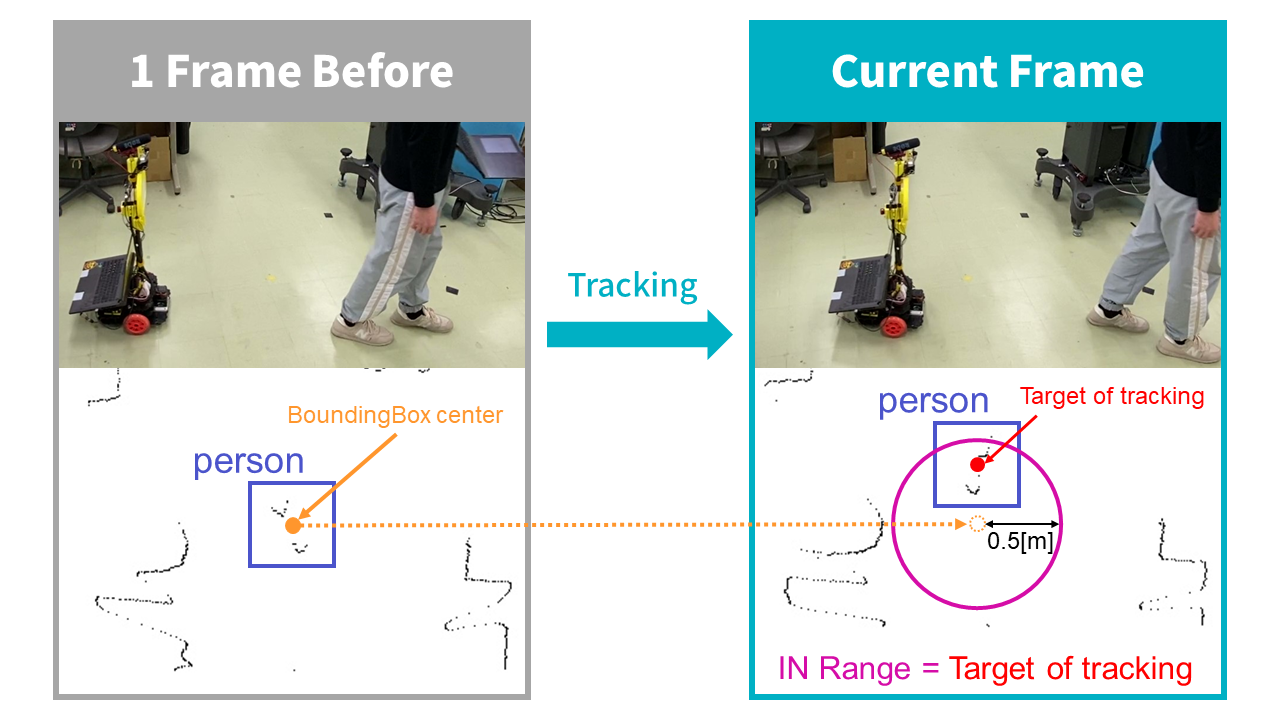
\includegraphics[height=100mm,clip]{figure/Target-identification-methods.png}
    \caption{Target identification methods}
    \label{Target identification methods}
    \end{center}
\end{figure*}

\clearpage

\section{ロボット台車の制御}
追従目標の特定により、追従目標のバウンディングボックスの中心から後方に定数で目標座標を生成
し、ロボットから目標座標までの距離と角度の偏差を収束させるためPID制御を実装した。 \\ \indent
時刻$t$での、ロボットの座標から目標座標までの角度の偏差を$\theta(t)$とし、ロボット台車の
エンコーダから取得できる旋回速度を$\omega(t)$とする。また、追従目標への角度の偏差が3.0[deg]
未満である場合に積分制御を開始する時刻を$t_1$としたとき、
ロボット台車の旋回速度の制御量$u_{angle}(t)$は以下のようになる。
\begin{equation}
\label{angularPID}
u_{angle}(t) = K_{AP} \cdot \theta(t)+ K_{AI} \cdot \int_{t_1}^{t-t_1} \theta(\tau) d\tau + K_{AD} \cdot \left\{ \frac{d}{dt} \theta(t) - \omega(t) \right\}
\end{equation}
$K_{AP}$、$K_{AI}$、$K_{AD}$は調整パラメータであり、$K_{AP}$は0.005、$K_{AI}$は0.0002、
$K_{AD}$は0.0009で設定している。(\ref{angularPID})式の第1項は、ロボットの座標から目標座標
までの角度の偏差を比例制御している。第2項は、ロボットが追従対象者の方向を定常偏差なく向く
ため、目標座標までの角度の偏差を積分制御している。第3項では、実機での制御を考慮し、
不足しているまたは過多な制御量を微分制御により調整している。積分制御を常にしていないのは、
角度の偏差が大きくなった場合に、積分値が時間経過に伴い過多になりすぎることで、
ロボットが左右に振動してしまうからである。\\ \indent
また、追従目標への距離の偏差を$l(t)$としたとき、ロボット台車の直進速度の制御量$u_{linear}(t)$
は以下のようになる。
\begin{equation}
\label{linearPID}
u_{linear}(t) = K_{LP} \cdot l(t)
\end{equation}
$K_{LP}$は調整パラメータである。(\ref{linearPID})式は、追従目標への距離の偏差を比例制御しており、
$K_{LP}$は0.3で設定している。

